
\\Our challenge for this application is to find the best available deals for the items in a given shopping list.  It will also be difficult to synchronize user profiles over various platforms, as indicated by the client wanting to be able to input recipes on one device, and using it on another.  Furthermore, there will be difficulties with concurrency issues regarding keeping prices up to date and managing recipes in databases.

The application will generally be broken into four parts: the front end, the back end, the database, and the data collection system.  The following is a brief overview of each system.
\begin{itemize}
    \item The front end of the application will have to be able to present fairly complex types of data, in terms of recipes, search results, application activity, and navigational information.
    \item The back end will have to handle user queries, such as item location/price searches and user profiles.  For the searches, it will be a relatively difficult task as the user will create a profile to indicate relative importance of distance versus cost for items, thus making it a nontrivial optimization problem.  In practice, there are various ways of solving this, but they will require a fairly computationally capable back end.
    \item The database will need to store all user information, such as shopping preferences and all recipes.  For the recipes, the application will require relational data as each recipe will have at least one step and ingredient, requiring the use of at least three tables.
    \item There will also be a data retrieval system, which will likely be a combination of web application programming interfaces (APIs) and web scraping tools.  This is highly dependant on the terms of service for the grocery stores being considered, as some of them allow web scraping while others only allow for access to be done through their API.
\end{itemize}
%\\We have decided to split the solution into three different parts: the front end, the back end and the database. Our front end will take a shopping list from the user, and the back end will find the best possible deal and give it back to the user. The best possible deal might be not be the cheapest item but it might be a deal that saves the user travel distance time at a slightly higher item price.\\
%\\Finally, the database is going to store various types of user data like login information, previous groceries list, etc.
% \begin{center}
\begin{figure}[h!]
    \centering
    \includegraphics[width=1\textwidth]{images/system_diagram.jpg}
    \caption{High level overview of the system}
\end{figure}
% \end{center}
% \begin{figure}[h!]
% 	\centering
%   	\includegraphics[width=1\textwidth]{project charter latex/images/system_diagram.jpg}
%   	\caption {High level overview of the system}
% \end{figure}

Another item that will have to be considered is security and authentication.  Since users will want their profiles to persist across platforms, it will be necessary to have some sort of login mechanic.  
For a rough outline of what the system architecture will look like, consider figure 1.


